\documentclass{beamer}
\usepackage[utf8]{inputenc}

\usepackage{semantic}
\usepackage{graphicx}
\usepackage{booktabs}
%\usepackage{todonotes}
\usepackage[absolute,overlay]{textpos}
\usepackage{tikz}
\usetikzlibrary{decorations.pathmorphing}

\mode<presentation> {
\usetheme{boxes} % When headline is wanted use Dresden theme instead
\usecolortheme{seagull}
\setbeamertemplate{footline}[page number]
\setbeamertemplate{navigation symbols}{}
}

%
% APL LaTeX declarations, based on work by A.Hohti/O.Kanerva
% University of Helsinki April 6 1987
%
% Written Oct. 3rd 2006 by Markus Triska (triska@gmx.at)
% Public domain code.

\font\apl=cmapl10 at 9pt      % The APL font of typewriter type

% from:
%		apldef.tex
%
% 2-letter control sequences for using cmapl10.
%===============================================================
%
\def\RO{{\apl\char'014}}               % rho
\def\IO{{\apl\char'015}}               % iota
\def\BX{\hskip0pt\lower.1ex\hbox{\apl\char'001}}               % quad box (window etc.)
\def\CE{{\apl\char'035}}               % ceiling
\def\FL{{\apl\char'034}}               % floor
\def\DE{{\apl\char'031}}               % decode
\def\EN{{\apl\char'030}}               % encode
\def\DL{{\apl\char'002}}               % del
\def\LD{{\apl\char'003}}               % delta
\def\NT{{\apl\char'026}}               % not
\def\LO{{\apl\char'017}}               % circle
\def\GO{{\apl\char'036}}               % arrow right
\def\OR{{\apl\char'010}}               % logical or
\def\DM{{\apl\char'011}}               % diamond
\def\LE{{\apl\char'012}}               % less than or equal
\def\GE{{\apl\char'013}}               % greater than or equal
\def\AB{{\apl\char'174}}               % stile
\def\LB{{\apl\char'173}}               % left brace
\def\RB{{\apl\char'175}}               % right brace
\def\DA{{\apl\char'037}}               % arrow down
\def\UA{{\apl\char'136}}               % arrow up
\def\EP{{\apl\char'006}}               % epsilon
\def\NE{{\apl\char'027}}               % not equal
\def\BL{{\apl\char'134}}               % backslash
\def\RU{{\apl\char'022}}               % right U
\def\LU{{\apl\char'023}}               % left U
\def\DU{{\apl\char'021}}               % down U
\def\UU{{\apl\char'020}}               % up U
\def\LK{{\apl\char'033}}               % right tack
\def\RK{{\apl\char'032}}               % left tack
\def\US{{\apl\char'024}}               % underscore
\def\NG{{\apl\char'025}}               % high minus
\def\DD{{\apl\char'007}}               % dieresis
\def\AM{{\apl\char'004}}               % alpha
\def\OM{{\apl\char'005}}               % omega
\def\SO{\leavevmode\raise.3ex\hbox{{\apl\char'016}}} % small circle
%
% This macro is used for overstriking two characters
\newskip\charwidth
\def\overstrike#1#2{\setbox1=\hbox{#1}\charwidth=\wd1
           #1\hskip-\charwidth#2}
%
\def\TR{\overstrike{\LO}{\BL}}                              % transpose
\def\RV{\overstrike{\LO}{\AB}}                              % reverse
\def\CR{\overstrike{\leavevmode\raise.1ex\hbox{\hskip0.361pt -}}{\LO}}
                                                   % column reverse
\def\GD{\overstrike{\DL}{\AB}}                              % grade down
\def\GU{\overstrike{\LD}{\AB}}                              % grade up
\def\FM{\overstrike{\leavevmode\raise.1ex\hbox{{\apl\char'016}}}{\EN}} % format
\def\XQ{\overstrike{\leavevmode\raise.1ex\hbox{{\apl\char'016}}}{\DE}} % execute
\def\SS{\overstrike{\RU}{\US}}                              % subset
\def\CO{\overstrike{\LU}{\US}}                              % contains
\def\CB{\overstrike{\BL}{-}}                                % column backslash
\def\CS{\overstrike{/}{-}}                                  % column slash
\def\IB{\overstrike{\EN}{\DE}}                              % I-beam
\def\DQ{\overstrike{{\apl\char'045}}{\BX}}                  % divide quad
\def\QQ{\overstrike{{\apl '}}{\BX}}                         % quote quad
\def\PD{\overstrike{\DL}{\NT}}                              % protected del
\def\NR{\overstrike{\OR}{\NT}}                              % nor
\def\NN{\overstrike{{\apl\char'046}}{\NT}}                  % nand
\def\LG{\overstrike{{\apl *}}{\LO}}                         % logarithm
\def\PO{\overstrike{\DD}{\apl *}}
% underscored letters
\def\ZA{\overstrike{{\apl A}}{\US}}
\def\ZB{\overstrike{{\apl B}}{\US}}
\def\ZC{\overstrike{{\apl C}}{\US}}
\def\ZD{\overstrike{{\apl D}}{\US}}
\def\ZE{\overstrike{{\apl E}}{\US}}
\def\ZF{\overstrike{{\apl F}}{\US}}
\def\ZG{\overstrike{{\apl G}}{\US}}
\def\ZH{\overstrike{{\apl H}}{\US}}
\def\ZI{\overstrike{{\apl I}}{\US}}
\def\ZJ{\overstrike{{\apl J}}{\US}}
\def\ZK{\overstrike{{\apl K}}{\US}}
\def\ZL{\overstrike{{\apl L}}{\US}}
\def\ZM{\overstrike{{\apl M}}{\US}}
\def\ZN{\overstrike{{\apl N}}{\US}}
\def\ZO{\overstrike{{\apl O}}{\US}}
\def\ZP{\overstrike{{\apl P}}{\US}}
\def\ZQ{\overstrike{{\apl Q}}{\US}}
\def\ZR{\overstrike{{\apl R}}{\US}}
\def\ZS{\overstrike{{\apl S}}{\US}}
\def\ZT{\overstrike{{\apl T}}{\US}}
\def\ZU{\overstrike{{\apl U}}{\US}}
\def\ZV{\overstrike{{\apl V}}{\US}}
\def\ZX{\overstrike{{\apl X}}{\US}}
\def\ZY{\overstrike{{\apl Y}}{\US}}
\def\ZW{\overstrike{{\apl W}}{\US}}
\def\ZZ{\overstrike{{\apl Z}}{\US}}

% unicode declarations

% first row
\DeclareUnicodeCharacter{22C4}{\DM} % diamond
\DeclareUnicodeCharacter{223C}{\NT} % not
\DeclareUnicodeCharacter{00A8}{\DD} % dieresis
\DeclareUnicodeCharacter{2336}{\IB} % I-Beam
\DeclareUnicodeCharacter{00AF}{\NG} % high minus
\DeclareUnicodeCharacter{236B}{\PD} % protected del
\DeclareUnicodeCharacter{2352}{\GD} % grade down
\DeclareUnicodeCharacter{2264}{\LE} % less than or equal
\DeclareUnicodeCharacter{234B}{\GU} % grade up
\DeclareUnicodeCharacter{233D}{\RV} % reverse
\DeclareUnicodeCharacter{2265}{\GE} % greater or equal
\DeclareUnicodeCharacter{2349}{\TR} % transpose
\DeclareUnicodeCharacter{2296}{\CR} % column reverse
\DeclareUnicodeCharacter{2260}{\NE} % not equal
\DeclareUnicodeCharacter{235F}{\LG} % logarithm
\DeclareUnicodeCharacter{2228}{\OR} % logical or
\DeclareUnicodeCharacter{2371}{\NR} % nor
\DeclareUnicodeCharacter{2227}{{\apl\char'046}} % and
\DeclareUnicodeCharacter{2372}{\NN} % nand
\DeclareUnicodeCharacter{00D7}{{\apl\char'043}} % times
\DeclareUnicodeCharacter{00F7}{{\apl\char'045}} % division
\DeclareUnicodeCharacter{2339}{\DQ} % divide quad / matrix division
% second row
\DeclareUnicodeCharacter{2375}{\OM} % omega
\DeclareUnicodeCharacter{2208}{\EP} % epsilon
\DeclareUnicodeCharacter{2377}{\overstrike{\EP}{\US}} % underscore epsilon
\DeclareUnicodeCharacter{2374}{\RO} % rho
\DeclareUnicodeCharacter{2191}{\UA} % up arrow
\DeclareUnicodeCharacter{2193}{\DA} % down arrow
\DeclareUnicodeCharacter{2373}{\IO} % iota
\DeclareUnicodeCharacter{2378}{\overstrike{\IO}{\US}} % underscore iota
\DeclareUnicodeCharacter{25CB}{\LO} % circle
\DeclareUnicodeCharacter{2365}{\overstrike{\DD}{\LO}} % circle dieresis
\DeclareUnicodeCharacter{22C6}{{\apl *}} % exponentiation
\DeclareUnicodeCharacter{235F}{\LG} % logarithm
\DeclareUnicodeCharacter{2190}{{\apl\char'137}} % arrow left
\DeclareUnicodeCharacter{2192}{\GO} % arrow right
\DeclareUnicodeCharacter{2340}{\CB} % column backslash
\DeclareUnicodeCharacter{2359}{\overstrike{\US}{\LD}} % delta underscore
% third row
\DeclareUnicodeCharacter{237A}{\AM} % alpha
\DeclareUnicodeCharacter{2296}{\CR} % column reverse
\DeclareUnicodeCharacter{2308}{\CE} % ceiling
\DeclareUnicodeCharacter{230A}{\FL} % floor
\DeclareUnicodeCharacter{2261}{$\equiv$}
\DeclareUnicodeCharacter{2207}{$\nabla$}
\DeclareUnicodeCharacter{2352}{\GD} % grade down
\DeclareUnicodeCharacter{2206}{\LD} % delta
\DeclareUnicodeCharacter{2218}{\SO} % jot
\DeclareUnicodeCharacter{2364}{\"\relax\hskip-5.8pt\SO} % jot dieresis
\DeclareUnicodeCharacter{233C}{\overstrike{\BX}{\LO}} % quad circle
\DeclareUnicodeCharacter{2395}{\BX} % quad
\DeclareUnicodeCharacter{235E}{\QQ} % quote quad
\DeclareUnicodeCharacter{22A2}{\LK} % right tack
\DeclareUnicodeCharacter{2342}{\overstrike{\BX}{\BL}} % quad backslash
\DeclareUnicodeCharacter{22A3}{\RK} % left tack
\DeclareUnicodeCharacter{233C}{\overstrike{\BX}{\LO}} % quad circle
\DeclareUnicodeCharacter{2282}{\RU} % right u
\DeclareUnicodeCharacter{2283}{\LU} % left u
\DeclareUnicodeCharacter{2229}{\DU} % down u
\DeclareUnicodeCharacter{235D}{{\apl\char'042}} % comment sign
\DeclareUnicodeCharacter{222A}{\UU} % up u
\DeclareUnicodeCharacter{22A5}{\DE} % decode
\DeclareUnicodeCharacter{234E}{\XQ} % execute
\DeclareUnicodeCharacter{22A4}{\EN} % encode
\DeclareUnicodeCharacter{2355}{\FM} % format
\DeclareUnicodeCharacter{2223}{\AB} % stile
\DeclareUnicodeCharacter{233F}{\CS} % column slash
\DeclareUnicodeCharacter{2212}{-}   % minus
\DeclareUnicodeCharacter{2262}{$\not\equiv$}
\DeclareUnicodeCharacter{220A}{\EP} % small contains, alternative for member
\DeclareUnicodeCharacter{2217}{{\apl *}} % asterisk, alternative for star
\DeclareUnicodeCharacter{03BA}{$\kappa$}
\DeclareUnicodeCharacter{2363}{\overstrike{\DD}{{\apl *}}}


%----------------------------------------------------------------------------------------
%	TITLE PAGE
%----------------------------------------------------------------------------------------

\title[FCL] % bottom of every slide
  {Introduction to GPU programming} % title page


\author{\footnotesize{Martin Dybdal} \\ \footnotesize{\texttt{dybber@dybber.dk}}}

\institute {
HIPERFIT research center \\
DIKU \\
University of Copenhagen
}

\date{\footnotesize{Workshop on Presentation techniques, 29 March 2016}}

% \title[Group Theory]{A longer title of the talk concerning Group Theory}
% \author[short name]{My full name}
% \institute[My Inst.]{Full Institut Name}
% % logo of my university

\date[4 March 2016]{4 March 2016}

\begin{document}

{
\setbeamertemplate{headline}{}
\begin{frame}
  \titlepage
\end{frame}
}

%----------------------------------------------------------------------------------------
%	TABLE OF CONTENTS
%----------------------------------------------------------------------------------------

% \begin{frame}
% \frametitle{Overview}
% \tableofcontents
% \end{frame}

%----------------------------------------------------------------------------------------
%	CONTENT
%----------------------------------------------------------------------------------------

\section{Motivation}

\begin{frame}
\frametitle{Physics simulation}
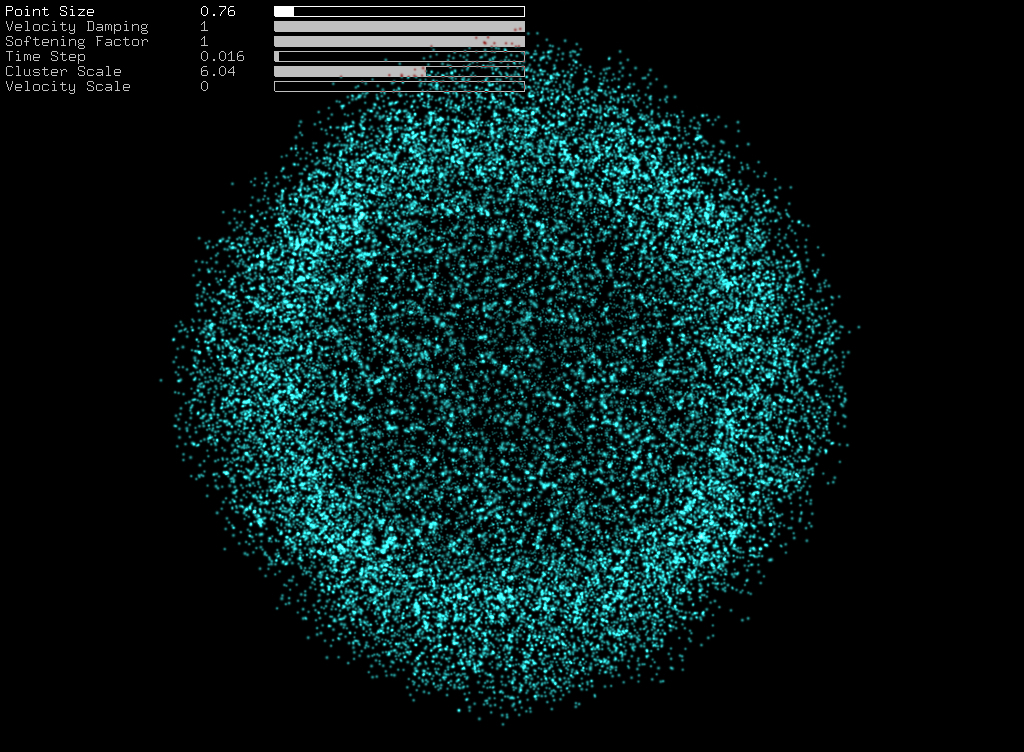
\includegraphics[width=\textwidth]{graphics/opencl_nbody}
\end{frame}

\begin{frame}
\frametitle{Financial simulation}
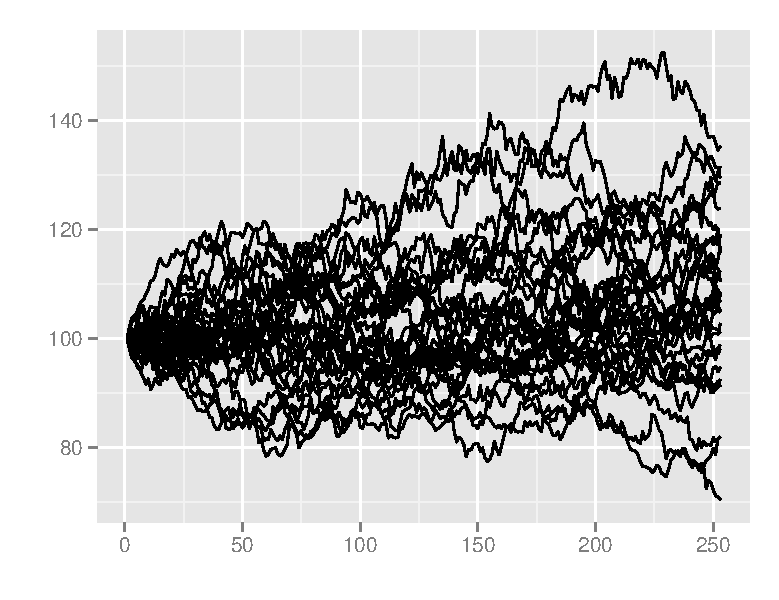
\includegraphics[width=\textwidth]{graphics/lsmplot}
\end{frame}

\tikzset{snake arrow/.style=
{-stealth,
decorate,
decoration={snake,amplitude=.4mm,segment length=2mm,post length=0.9mm}},
}

\section{CPU vs. GPU}

\begin{frame}[fragile]
\frametitle{Standard CPU}
\only<1-3>{
\begin{tikzpicture}
\begin{scope}[every edge/.append style = {snake arrow}]
\node  at (0,2.5) {\footnotesize Core 0}; 
\node  at (1.25,2.5) {\footnotesize Core 1}; 
\node  at (2.5,2.5) {\footnotesize Core 2}; 
\node  at (3.75,2.5) {\footnotesize Core 3}; 
\draw (0,2) edge (0,0)
      (1.25,2) edge (1.25,0)
      (2.5,2) edge (2.5,0)
      (3.75,2) edge (3.75,0);
\end{scope}
\end{tikzpicture}
}
\only<4->{
\begin{tikzpicture}
\begin{scope}[every edge/.append style = {snake arrow}]
\node  at (0,2.5) {\footnotesize Core 0}; 
\node  at (1.25,2.5) {\footnotesize Core 1}; 
\node  at (2.5,2.5) {\footnotesize Core 2}; 
\node  at (3.75,2.5) {\footnotesize Core 3}; 
\draw (0,1) edge (0,0)
      (0,2) edge (0,1)
      (1.25,0.66) edge (1.25,0)
      (1.25,1.33) edge (1.25,0.66)
      (1.25,2) edge (1.25,1.33)
      (2.5,2) edge (2.5,0)
      (3.75,2) edge (3.75,0);
\end{scope}
\end{tikzpicture}
}
\only<5->{
\begin{textblock*}{6cm}(6.5cm,2cm)
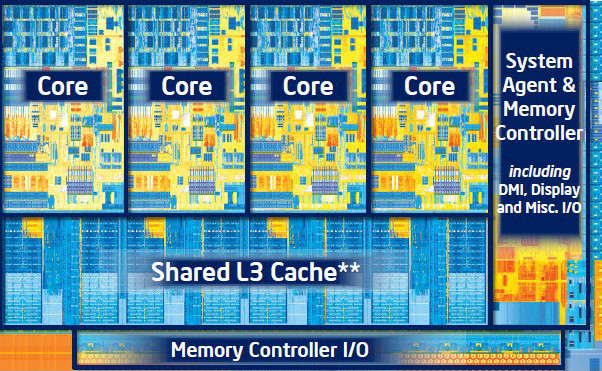
\includegraphics[width=\textwidth]{graphics/ivybridge.jpg}
\end{textblock*}
}
\vspace{3mm}
\begin{itemize}
\item<2-> One operation at a time
\item<3-> Few compute units (cores)
\item<4-> Fast at switching between tasks
\item<5-> Most transistors used for ``recalling''
\end{itemize}

\end{frame}

\begin{frame}[fragile]
\frametitle{GPU}
\begin{tikzpicture}
\begin{scope}[every edge/.append style = {snake arrow}]
\foreach \x in {0,...,16}
  \draw (0.25*\x,1) edge (0.25*\x,0);
\end{scope}
\foreach \y in {0,...,4}
  \draw [color=lightgray](0,0.2+0.2*\y) edge (4,0.2+0.2*\y);
%\draw [color=gray,thick](-0.25,-0.25) rectangle (4.25,1.25);
\end{tikzpicture}

% \vspace{2mm}
% \begin{tikzpicture}
% \begin{scope}[every edge/.append style = {snake arrow}]
% \foreach \x in {0,...,16}
%   \draw (0.25*\x,1) edge (0.25*\x,0);
% \end{scope}
% \foreach \y in {0,...,4}
%   \draw [color=lightgray](0,0.2+0.2*\y) edge (4,0.2+0.2*\y);
% %\draw [color=gray,thick](-0.25,-0.25) rectangle (4.25,1.25);
% \end{tikzpicture}

\vspace{10mm}

\begin{textblock*}{4cm}(8.2cm,1cm)
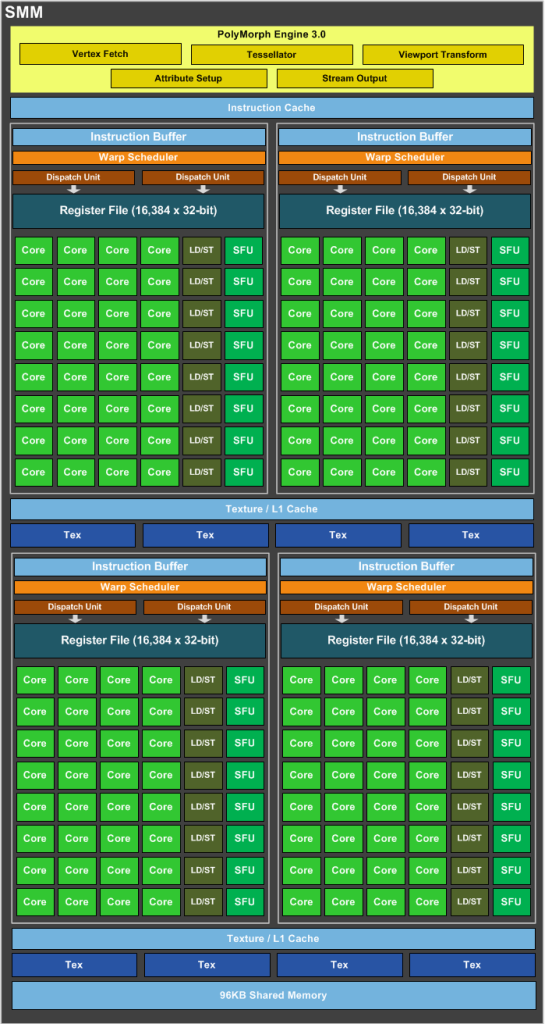
\includegraphics[width=\textwidth]{graphics/gtx980}
\end{textblock*}

\begin{itemize}
\item<2-> Identical operations on diff. data
\item<3-> Thousands of compute units (cores)
\item<4-> Tasks executed in order (queued)
\item<5-> Most transistors used for computing
\end{itemize}

\end{frame}

\begin{frame}[fragile]
\frametitle{CPU vs. GPU programming}

\begin{textblock*}{0.6\textwidth}(0.1\textwidth,2cm)
CPU programming
\begin{verbatim}
5+9
      14
14+3
      17
17+22
      39
\end{verbatim}
\end{textblock*}

\begin{textblock*}{0.7\textwidth}(0.5\textwidth, 2cm)
GPU programming
\begin{verbatim}
(2 4 6 8 10) + 100
      102 104 106 108 110

(102 104 106 108 110) * 2
      204 208 212 216 220
\end{verbatim}
\end{textblock*}
\end{frame}

\begin{frame}[fragile]
\frametitle{GPU programming}

Problem:
\begin{itemize}
\item GPU cores are bad at ``recalling''
\item manual control of ``scratch pad''
\end{itemize}

\end{frame}

\begin{frame}[fragile]
\frametitle{Fusion}

\begin{verbatim}
((2 4 6 8 10) + 100) * 2
      204 208 212 216 220
\end{verbatim}
\end{frame}

\begin{frame}
\frametitle{Summary}
\begin{itemize}
\item GPUs require many similar computations on different data
\item GPUs require attention to memory transactions (fusion)
\item GPU programming: as hard as programming CPUs in the 60s/70s
\end{itemize}
\end{frame}


\end{document}